\chapter{Pomiarowa weryfikacja tezy}

Ostatnim etapem weryfikacji postawionej w pracy tezy będzie analiza właściwości metrologicznych przykładowego toru pomiarowego, który stworzony został na potrzeby pracy. Analizowany tor pomiarowy przetwarzać będzie zmienny w czasie sygnał napięciowy $s(t)$ o chwilowej wartości napięcia z przedziału $<0;1>~\unit{V}$. W celu dopasowania poziomu sygnału napięcia wejściowego do zakresu napięcia wejściowego przetwornika analogowo-cyfrowego oraz zwiększenia impedancji wejściowej toru pomiarowego, sygnał $s(t)$ podawany będzie na wejście wzmacniacza pomiarowego. Sygnał wyjściowy wzmacniacza $y(t)$ przetwarzany będzie na postać cyfrową $c(i)$, a następnie po wykonaniu odtwarzania statycznego, podawany będzie w postaci wielkości $x(i)$ na wejście jednostki \enquote{DSP}, która pobierać będzie $N$ próbek tego sygnału i wyznaczać na ich podstawie $M$ wartości wielkości wyjściowych toru pomiarowego, stosując w tym celu algorytm dyskretnej transformacji falkowej. Schemat blokowy omawianego toru pomiarowego przedstawiono na rysunku~\ref{fig:chain_real}.

\begin{figure}[htb!]
\begin{center}
\includegraphics{obrazki/schemat_real}
\makecaption{fig:chain_real}{Schemat blokowy stworzonego na potrzeby pracy toru pomiarowego będącego obiektem przeprowadzanego eksperymentu}
\end{center}
\end{figure}

Do realizacji układu wzmacniacza pomiarowego zastosowany został wzmacniacz operacyjny \enquote{MCP6002} w konfiguracji nieodwracającej, o docelowym wzmocnieniu wynoszącym~\qty{3.3}{V \per V}. Napięcie zasilania wzmacniacza wynosi~\qty{3.3}{V} i pochodzi ze stabilizatora \enquote{LD1117} typu \enquote{LDO} (ang. \enquote{Low Dropout}). Zaproponowana konfiguracja, zgodnie z wcześniejszymi założeniami, zapewnia wysoką impedancję wejściową toru pomiarowego oraz bardzo niską impedancję wyjściową wzmacniacza. Parametry statyczne oraz dynamiczne analizowanego obiektu wymagają identyfikacji, ze względu na niedostateczne informacje zawarte w dokumentacji wykorzystanego układu oraz nieznajomości dokładnego modelu dla zastosowanej aplikacji. Należy zauważyć, że dokładna analiza zastosowanego układu byłaby skomplikowana i nie jest konieczna do oceny jego podstawowych właściwości metrologicznych.

Zastosowany przetwornik analogowo-cyfrowy stanowi $12$-bitowy przetwornik wagowy~\enquote{SAR} (ang. \enquote{Successive Approximation Register}), wbudowany w mikrokontroler \enquote{STM32F411}. Źródło napięcia odniesienia stanowi w jego przypadku stabilizator \enquote{LD3985} typu \enquote{ULD} (ang. \enquote{Ultra Low Dropout}), o znamionowym napięciu wyjściowym równym~\qty{3.3}{V}, przyłączony z użyciem dodatkowego filtru LR. Przetwornik taktowany jest wewnętrznym sygnałem zegarowym o częstotliwości~\qty{24}{MHz}, przy czym próbkowanie wyzwalane jest sygnałem z licznika, którego częstotliwość wyzwalania wynosi~\qty{48}{kHz}. Częstotliwość próbkowania analizowanego toru pomiarowego wynosi zatem $f_{s} = \qty{48}{kHz}$. Na proces konwersji analogowo-cyfrowej przypada proces kluczowania napięcia wejściowego trwający TODO taktów zegara, co odpowiada czasowi~\qty{123}{ns}, po którym następuje konwersja trwająca $15$ taktów zegara, co w analizowanym przypadku stanowi czas~\qty{625}{ns}. Łączny czas konwersji analogowo-cyfrowej pojedynczej próbki sygnału wejściowego $y(t)$ na jego dyskretną reprezentację $c(i)$ wynosi zatem~\qty{1234}{ns}. Ze względu na typową aplikacje omawianego przetwornika, jego parametry metrologiczne mogą zostać pozyskane z dokumentacji producenta układu.

Pozyskane próbki napięcia $x(i)$, stanowiące dyskretną reprezentację sygnału wejściowego $s(t)$, zapisywane są w wektorze $\mathbf{x}$ o długości $N = 128$. Wektor wielkości wejściowych $\mathbf{x}$ podawany jest na wejście algorytmu dyskretnej transformacji falkowej, którego implementacja zrealizowana jest z wykorzystaniem instrukcji \enquote{DSP} zastosowanego mikrokontrolera. Analizowany algorytm wykorzystuje falkę \enquote{spline4:4} dla pięciu iteracji procesu dekompozycji sygnału. Zgodnie z równaniem~\eqref{eq:alg_out_mat} wyznaczanych jest $M = 128$ próbek wektora wielkości wyjściowych $\mathbf{X}$, które stanowią wyjście pojedynczej serii pomiarowej analizowanego toru pomiarowego. Czas obliczeń wynosi w analizowanym przypadku~\qty{1508}{\micro s}, przy czym łączny czas akwizycji pojedynczego wektora próbek wielkości wejściowych wynosi~\qty{2666.6(6)}{\micro s}.

Przedstawiony tor pomiarowy pracuje w trybie ciągłym, tj. w pojedynczym oknie pomiarowym, podczas pobierania próbek wielkości wejściowych, wyznaczana jest realizacja wektora wielkości wyjściowych dla poprzedniej realizacji wektora wielkości wejściowych. Wykorzystywany jest w tym celu kontroler \enquote{DMA} (ang. \enquote{Direct Memory Access}), nadzorujący proces buforowania kolejnych realizacji sygnału $x(i)$, w czasie gdy program główny wykonuje obliczenia. Analiza wartości wielkości wyjściowych omawianego toru pomiarowego jest możliwa między innymi po podłączeniu go do komputera klasy \enquote{PC} za pośrednictwem portu \enquote{USB}, przy czym wykorzystywany jest w tym celu układ peryferyjny \enquote{USB OTG Full-Speed}, zintegrowany w zastosowanym mikrokontrolerze.

W dalszej części rozdziału zidentyfikowane zostaną najważniejsze źródła błędów analizowanego toru pomiarowego, a następnie wykorzystany zostanie zaproponowany w pracy model błędu do opisu właściwości wykazanych sygnałów błędów. Ze względu na fakt, że nie jest znany dokładny model analizowanego toru pomiarowego, zostanie przedstawiona metoda identyfikacji jego właściwości, istotnych ze względu na zaproponowany model błędu i jego aplikację. W ostatniej części rozdziału przeprowadzony zostanie eksperyment pomiarowy, wykorzystujący metodę Monte-Carlo, mający na celu ocenę poprawności przedstawionych rozważań i weryfikacje możliwości praktycznej aplikacji zawartych w pracy propozycji. Podczas eksperymentu przyjmuje się, że temperatura otoczenia będzie stała i wynosić będzie~\qty{20}{\degreeCelsius}. Stosowanym podczas eksperymentu źródłem napięcia wielkości wejściowej $s(t)$ będzie generator przebiegów arbitralnych RIGOL~DG1011~\cite{rigol_manual}.

\section{Identyfikacja właściwości toru pomiarowego}

Pierwszą grupą identyfikowanych właściwości analizowanego toru pomiarowego będą jego właściwości statyczne. Właściwości te nie zależą od częstotliwości przetwarzanego sygnału i wynikać będą z charakterystyk przetwarzania statycznego kolejnych fragmentów tego toru. Jako, że z punktu widzenia przeprowadzanej analizy właściwości metrologicznych oraz właściwości zaproponowanej w pracy metody analizy, najistotniejsze informacje stanowić będą dane dotyczące parametrów sygnałów błędów na wejściu algorytmu dyskretnej transformacji falkowej, najbardziej przystępne z punktu widzenia projektanta toru pomiarowego będzie wyznaczenie tych parametrów traktując całość toru pomiarowego znajdującego się przed tym algorytmem, jak jeden obiekt.

Wobec powyższych, proponuje się wyznaczenie charakterystyki statycznej $f_{c}(x)$ dla wielkości wyjściowej $c(i)$ przetwornika analogowo-cyfrowego, a następnie na jej podstawie określenie funkcji odtwarzania $f_{x}(x)$. Należy w tym celu na wejście toru pomiarowego podawać, z wzorcowego źródła napięcia, napięcie stałe o zadanej wartości, a następnie pobierać wielokrotnie wartość realizacji wielkości wyjściowej przetwornika analogowo-cyfrowego, którą następnie należy uśrednić dla przeprowadzonej serii pomiarów. W eksperymencie przyjmuje się, że na wejście toru pomiarowego podawane będzie napięcie stałe z zakresu $<25;975>~\unit{mV}$ z krokiem wynoszącym~\qty{50}{mV}, a na pojedynczą serię pomiarową składać się będzie trzydzieści tysięcy próbek wielkości wyjściowej przetwornika analogowo-cyfrowego. Uzyskaną w opisywany sposób charakterystykę przedstawiono na rysunku~\ref{fig:pom_static_fun}.

\begin{figure}[htb!]
\begin{center}
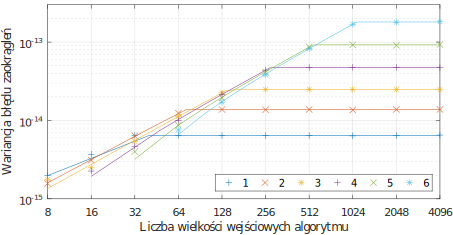
\includegraphics{obrazki/dwt_rerror_coif5}
\makecaption{fig:pom_static_fun}{Zależność wartości wielkości wyjściowej przetwornika analogowo-cyfrowego w funkcji wartości napięcia wejściowego analizowanego toru pomiarowego}
\end{center}
\end{figure}

Na podstawie uśrednionych wartości wyników pomiarów, po wykonaniu aproksymacji liniowej stosując metodę najmniejszych kwadratów, funkcję przetwarzania analizowanego obiektu opisać można równaniem:
\begin{equation}
c \emb{i} = f_{c} \emb{s(iT_{p}} = 123.4 \cdot s \emb{iT_{p}} \label{eq:pom_func_static}.
\end{equation}
Zakładając, że czułość wielkości $x(i)$ równa będzie~\qty{1}{V \per V}, funkcja odtwarzania statycznego dla wielkości $x(i)$ jest dana następującym równaniem:
\begin{equation}
x \emb{i} = f_{x} \emb{c \emb{i}} = 123.4 \cdot c \emb{i} \label{eq:pom_funx_static}.
\end{equation}

Dodatkowo uwzględnić należy podczas analizy występowanie czynników zakłócających proces pomiaru, których charakter określić można jako losowy. W omawianej grupie mieścić się będą zakłócenia wynikające przede wszystkim z fluktuacji napięcia zasilania oraz odniesienia, błędu kwantowania oraz nieliniowości zastosowanych obiektów, a także szumów występujących w części analogowej toru pomiarowego. Cennym źródłem informacji będzie zatem histogram przedstawiający uzyskane realizacje błędu odtwarzania wielkości $s(t)$, opisanego równaniem:
\begin{equation}
e_{x} \emb{i} = x \emb{i} - s \emb{iT_{p}} \label{eq:pom_funx_error}.
\end{equation}
Uzyskany histogram dla pozyskanych wcześniej danych pomiarowych przedstawiono na rysunku~\ref{fig:pom_static_hist}. Zidentyfikowane właściwości posłużą w dalszej części rozdziału do budowy modelu błędu wskazanego toru pomiarowego.

\begin{figure}[htb!]
\begin{center}
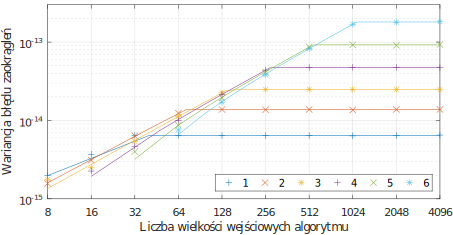
\includegraphics{obrazki/dwt_rerror_coif5}
\makecaption{fig:pom_static_hist}{Zależność wartości wielkości wyjściowej przetwornika analogowo-cyfrowego w funkcji wartości napięcia wejściowego analizowanego toru pomiarowego}
\end{center}
\end{figure}

Drugą grupą koniecznych do identyfikacji właściwości są właściwości dynamiczne. Podobnie, jak w przypadku właściwości statycznych, istnieje możliwość ich identyfikacji pomiarowej uzyskując kolejne realizacje wielkości wyjściowej $c(i)$. Przypadek właściwości dynamicznych jest jednak bardziej skomplikowany i wymagałby w tym przypadku bardziej skomplikowanej procedury pomiarów -- konieczna bowiem byłaby odpowiednia synchronizacja przebiegu napięcia sygnału wejściowego toru pomiarowego z wyjściem przetwornika analogowo-cyfrowego. Opisywana procedura byłaby zatem kłopotliwa, a dodatkowo do pomiaru zostałby wprowadzony kolejny błąd związany z opisywaną synchronizacją. Proponuje się zatem w pierwszej kolejności zidentyfikować właściwości zastosowanego wzmacniacza, a następnie ustalić właściwości przetwornika analogowo cyfrowego na podstawie jego dokumentacji.

W przypadku wzmacniacza pomiarowego procedura identyfikacji polegać będzie na podawaniu na jego wejście napięcia sinusoidalnie zmiennego o zadanej częstotliwości i stałej amplitudzie. Dla zadanych parametrów sygnału zmierzyć należy amplitudę sygnału wyjściowego wzmacniacza, potrzebną do wyznaczenia jego wzmocnienia $K_{y}(f)$, oraz przesunięcie fazowe $\varphi_{y}(t)$ pomiędzy sygnałem wejściowym $s(t)$ i wyjściowym $y(t)$, przy czym pomiędzy omawianymi wielkościami zachodzą następujące relacje:
\begin{gather}
K_{y} \emb{f} = 20 \log \left( \frac{A_{wy} \emb{f}}{A_{we} \emb{f}} \right) \label{eq:pom_dyn_amp}, \\
\varphi_{y} \emb{f} = \varphi_{wy} \emb{f} - \varphi_{we} \emb{f} \label{eq:pom_dyn_phi},
\end{gather}
gdzie w funkcji częstotliwości $A_{wy}(f)$ jest amplitudą sygnału wyjściowego, $A_{we}(f)$ amplitudą sygnału wejściowego, $\varphi_{wy}(f)$ przesunięciem fazowym sygnału napięcia wyjściowego, natomiast $\varphi_{we}(f)$ przesunięciem fazowym sygnału napięcia wejściowego analizowanego wzmacniacza.

Na podstawie pozyskanych danych oszacować można częstotliwość graniczną analizowanego wzmacniacza, która w tym przypadku wyniosła $f_{y,g} = \qty{123}{kHz}$. Dla przedstawionych charakterystyk sporządzono dwa modele aproksymacji. W modelu pierwszym wykorzystano funkcję opisującą transmitancję wzmacniacza w postaci:
\begin{gather}
\tilde{G}_{y} \emb{j\omega} = \frac{1}{1 + j \frac{\omega}{2 \pi f_{y,g}}} = \frac{1}{\frac{\omega^{2}}{4 \pi^{2} f_{y,g}^{2}} + 1} - j \frac{\omega}{2 \pi f_{y,g} \left( \frac{\omega^{2}}{4 \pi^{2} f_{y,g}^{2}} + 1 \right) } \label{eq:pom_dyn_trans},
\end{gather}
natomiast dla modelu drugiego wykonano metodą najmniejszych kwadratów aproksymacje wielkości danych równaniami~\eqref{eq:pom_dyn_amp} oraz~\eqref{eq:pom_dyn_phi} przy użyciu wielomianów:
\begin{gather}
K_{y} \emb{f} = 123 \cdot f^{2} - 321 \cdot f \label{eq:pom_aprox_amp}, \\
\varphi_{y} \emb{f} = 123 \cdot f^{2} - 321 \cdot f \label{eq:pom_aprox_phi}.
\end{gather}
Uzyskane dla zakresu częstotliwości $<0.1;300>~\unit{kHz}$ wartości wzmocnienia i przesunięcia fazowego oraz odpowiadające im wartości dla zaproponowanych w równaniach od~\eqref{eq:pom_dyn_trans} do~\eqref{eq:pom_aprox_phi} przedstawiono na rysunkach~\ref{fig:pom_dynamic_amp} oraz~\ref{fig:pom_dynamic_phi}.

\begin{figure}[htb!]
\begin{center}
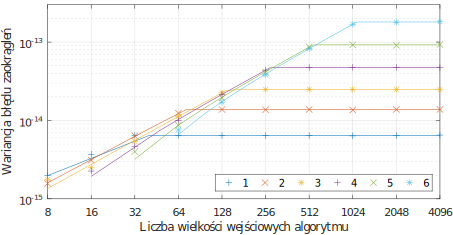
\includegraphics{obrazki/dwt_rerror_coif5}
\makecaption{fig:pom_dynamic_amp}{Zależność wartości wzmocnienia w funkcji częstotliwości dla zastosowanego w torze pomiarowym wzmacniacza}
\end{center}
\end{figure}

\begin{figure}[htb!]
\begin{center}
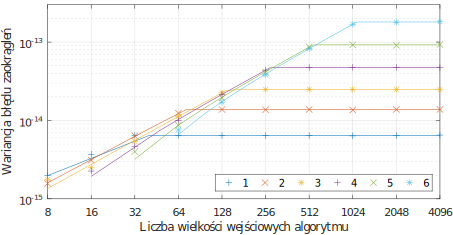
\includegraphics{obrazki/dwt_rerror_coif5}
\makecaption{fig:pom_dynamic_phi}{Zależność wartości przesunięcia fazowego w funkcji częstotliwości dla zastosowanego w torze pomiarowym wzmacniacza}
\end{center}
\end{figure}

Analizując przedstawione wykresy zauważyć można, że model zaproponowany w równaniach~\eqref{eq:pom_aprox_amp} oraz~\eqref{eq:pom_aprox_phi} stanowi bardzo dobre przybliżenie charakterystyki analizowanego wzmacniacza pomiarowego, natomiast model dany równaniem~\eqref{eq:pom_dyn_trans} odbiega od niej znacząco. Stąd, w dalszej części rozdziału przyjmuje się, że omawiane równania~\eqref{eq:pom_aprox_amp} oraz~\eqref{eq:pom_aprox_phi} opisywać będą właściwości dynamiczne zastosowanego wzmacniacza, odpowiadające zależnościom~\eqref{eq:mid_cont_amp} oraz~\eqref{eq:mid_cont_phi}. Należy zauważyć, że na potrzeby zaproponowanego w pracy modelu błędu informacje te będą wystarczające i nie jest konieczna znajomość dokładnej postaci funkcji opisującej transmitancję analizowanego obiektu.

Zgodnie z dokumentacją~\cite{stm_f411} obwód zastępczy części analogowej przetwornika analogowo-cyfrowego przedstawić można w postaci modelu filtra dolno-przepustowego typu \enquote{RC}, przy czym stanowić on będzie kaskadowe połączenie dwóch takich filtrów, co przedstawiono na rysunku~\ref{fig:schemat_adc}. Wypadkowa pojemność $C_{we}$ wynika w analizowanym przypadku z pojemności w obrębie wyprowadzenia mikrokontrolera, natomiast pojemność $C_{adc}$ wynika pojemności wewnętrznej układu próbkująco-pamiętającego. Zgodnie z dokumentacją wewnętrzna pojemność przetwornika wynosi typowo około~\qty{4}{pF}, natomiast pojemność wynikająca z wyprowadzenia oraz zastosowanego laminatu wynosi około~\qty{5}{pF}. Rezystancję $R_{we}$ w zaproponowanym modelu stanowi szeregowe połączenie rezystancji doprowadzeń pomiędzy wzmacniaczem pomiarowym i mikrokontrolerem oraz rezystancja samego wzmacniacza, przy czym w omawianym przypadku jest to wartość rzędu pojedynczych Ohmów. Rezystancja $R_{adc}$ jest rezystancją klucza układu próbkująco-pamiętającego i, zgodnie z dokumentacją, jej wartość nie przekracza~\qty{6}{k\ohm}. Dodatkowe elementy, które można zauważyć na omawianym schemacie, to diody zabezpieczające wejście mikrokontrolera przed zbyt wysokim lub niskim napięciem oraz źródło $I_{adc}$, które zastępuje upływność nieprzekraczającą~\qty{\pm 1}{\micro A}. Elementy te mogą być zatem pominięte w omawianej analizie.

\begin{figure}[htb!]
\begin{center}
\includegraphics{obrazki/schemat_adc}
\makecaption{fig:schemat_adc}{Schemat zastępczy modelu przetwornika analogowo-cyfrowego zastosowanego w analizowanym torze pomiarowym}
\end{center}
\end{figure}

Pierwszy filtr, który przedstawiono na rysunku~\ref{fig:schemat_adc}, składa się z rezystancji rzędu pojedynczych Ohmów oraz pojemności rzędu mikro Faradów. Pozwala to oszacować częstotliwość graniczną tego filtru na poziomie kilkuset giga Herców. Filtr drugi stanowi połączenie rezystancji rzędu kilo Ohmów z pojemnością rzędu piko Faradów, a zatem rząd wielkości częstotliwości granicznej takiego filtru oszacować można na poziomie kilkuset mega Herców. Na podstawie przedstawionych parametrów modelu analizowanego przetwornika analogowo-cyfrowego, przyjąć można pomijalnie mały udział jego parametrów dynamicznych w puli właściwości dynamicznych całego toru pomiarowego. Ostateczna analiza właściwości dynamicznych całości toru pomiarowego uwzględniać będzie jedynie właściwości zastosowanego wzmacniacza pomiarowego, którego częstotliwość graniczna cechowała się wartością rzędu kilkuset kilo Herców.

Ostatnim fragmentem toru pomiarowego, który wprowadzać może do sygnału wyjściowego dodatkowe błędy, jest algorytm dyskretnej transformacji falkowej. Jako, że zastosowany mikrokontroler posiada jednostkę \enquote{FPU} (ang. \enquote{Floating Point Unit}) oraz zestaw instrukcji \enquote{DSP} umożliwiające optymalne wykonywanie operacji na liczbach zmiennoprzecinkowych pojedynczej precyzji, wykorzystane zostaną liczby o długości słowa $32$-bitów. Przeprowadzone wcześniej badania, których wyniki przedstawiono w tabeli~\ref{tab:varnum_spline4_4_5_f32} pozwalają przypuszczać, że wariancja błędu związanego z zaokrągleniami nie przekroczy w bieżącym przypadku rzędu piko Voltów, a zatem niepewność rozszerzona z nią związana nie przekroczy rzędu mikro Voltów.

Dotychczasowe rozważania zakładały, że podawany na wejście toru pomiarowego z zastosowanego generatora sygnał cechował się idealną wartością napięcia. W rzeczywistości sygnał ten również obarczony był pewnym błędem, który zostanie uwzględniony i opisany w kolejnym podrozdziale. Przedstawione dotychczas zabiegi umożliwią sporządzenie modelu błędu analizowanego toru pomiarowego w oparciu o model błędu przedstawiony w niniejszej pracy.

\section{Model błędu toru pomiarowego}

TODO

\section{Weryfikacja przedstawionych zależności}

TODO

\section{Podsumowanie przeprowadzonego eksperymentu}

TODO

